%!TeX root=../tese.tex
%(dica para o editor de texto: este arquivo é parte de um documento maior)
% para saber mais: https://tex.stackexchange.com/q/78101/183146

\chapter{Procedimentos de comparação e resultados}
\label{cap:comparacao}

Neste capítulo serão definidos procedimentos de modelagem alternativos às séries temporais financeiras de taxas de câmbio. Um dos modelos é o modelo paramétrico \eng{ARIMA}, estudado no Capítulo \ref{cap:series}. 

O outro será um modelo não-paramétrico criado com redes neurais, estudadas no Capítulo \ref{cap:perceptron}, sendo utilizadas redes neurais recorrentes, devido à sua arquitetura mais condizente com o problema em questão, de acordo com Kopec \citep{classic} e Géron \citep{hands}.

A seguir, serão feitas comparações entre os modelos preditivos de séries temporais, através de medidas de desempenho comuns como as funções de erros RMSE\footnote{Raiz do erro quadrático médio} e MAE\footnote{Erro absoluto médio} e a correlação entre os valores previstos e conhecidos do conjunto de teste.

\section{Modelagem e procedimentos}

A princípio, foi escolhido um período com os valores em Reais de cotações de venda do Dólar. Esse período de dados foi dividido em \emph{janelas de dados} móveis e de tamanho fixo. Considere o seguinte exemplo. 

Seja a sequência de números de $0$ a $9$: $(0,1,2,3,4,5,6,7,8,9)$. Suponha que queremos criar janelas de dados de tamanho $6$, elas seriam uma sequência de sequências:
\[ ((0,1,2,3,4,5),(1,2,3,4,5,6),(2,3,4,5,6,7),(3,4,5,6,7,8),(4,5,6,7,8,9)) \]

Perceba que criamos, a partir da sequência de $10$ números original, $5$ janelas com $6$ números cada, o tamanho de cada uma. Generalizando, se temos $N$ dados, podemos criar $N{-}M{+}1$ janelas de dados de tamanho $M$.

A ideia geral é usar essas janelas de dados para treinar modelos que descrevam a série de cotações. Numa série temporal financeira, temos os valores passados, e podemos querer prever valores futuros apenas com as informações que temos do passado.

Após download do arquivo CSV com os valores de cotação do Dólar, obtido no site do Banco Central do Brasil\footnote{\url{https://olinda.bcb.gov.br/olinda/servico/PTAX/versao/v1/aplicacao}}, filtrei para um período específico, que vai de Julho/2016 até Dezembro/2017, ou seja, totalizando $18$ meses de dados. Essa série temporal está listada na Figura \ref{fig:serie_1}, abaixo.

\begin{figure}[htb]
\centering
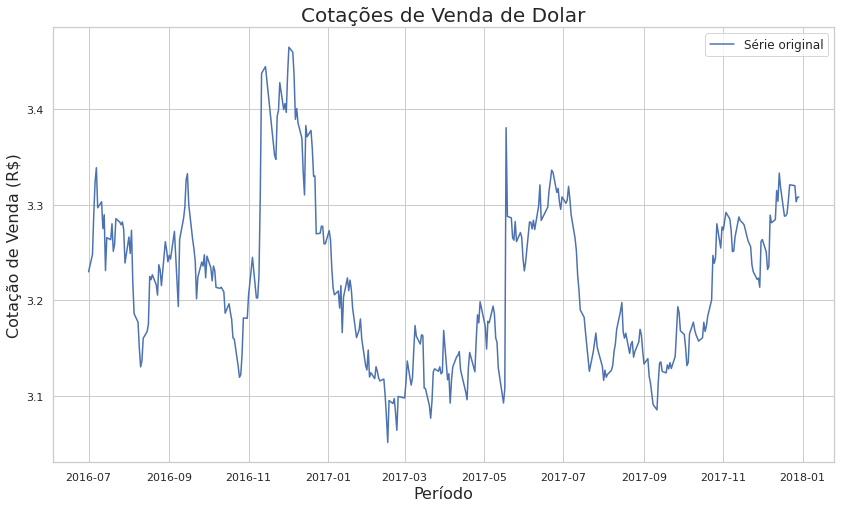
\includegraphics[width=14cm]{figuras/serie_1}
\caption{Cotações de venda do Dólar em Reais. Período: Jul/2016 - Dez/2017.}
\label{fig:serie_1}
\end{figure}

De forma a treinar os modelos de forma mais justa, foi definido que serão utilizadas janelas de $30$ dias de valores de câmbios passados para prever o valor de câmbio do dia imediatamente a seguir. Por exemplo, suponha que tenhamos uma janela com valores dos $30$ dias de Junho, essa janela será uma série temporal que será modelada e então cada modelo irá prever a taxa de câmbio do dia $1$° de Julho.

Isto não está exato, pois a série não possui dados para cada dia do ano, apenas para dias úteis, pulando finais de semana e feriados. Na prática, escolhi prever os valores da série no período que vai de $16/08/2017$ até $24/08/2017$. 

Dessa forma, utilizando as janelas de $30$ dias passados, de acordo com os dias úteis disponíveis, criei as $7$ janelas, sendo que a primeira tem seus $30$ valores contidos no período de $05/07/2017$ a $15/08/2017$, e assim sucessivamente para as próximas janelas.

\emph{Vou explicar mais coisas aqui...}

\begin{table}[]
\begin{center}
\begin{tabular}{|c|c|c|c|c|}
\hline
\multirow{2}{*}{\textbf{Dia}} & \multirow{2}{*}{\textbf{Cotação}} & \multirow{2}{*}{\textbf{ARIMA}} & 
\textbf{Rede Neural} & \textbf{Rede Neural} \\
&&& \textbf{(Keras)} & \textbf{(Perceptron)} \\
\hline
\hline
16/08/2017 & 3.1670 & 3.2039 & 3.1770 & 3.1976 \\
17/08/2017 & 3.1603 & 3.1505 & 3.1737 & 3.1402 \\
18/08/2017 & 3.1654 & 3.1584 & 3.1694 & 3.1976 \\
21/08/2017 & 3.1443 & 3.1690 & 3.1632 & 3.1402 \\
22/08/2017 & 3.1539 & 3.1370 & 3.1592 & 3.1402 \\
23/08/2017 & 3.1569 & 3.1589 & 3.1561 & 3.1402 \\
24/08/2017 & 3.1404 & 3.1584 & 3.1534 & 3.1402 \\
\hline
\hline
\textbf{MAE} & - & 0.0165 & 0.0093 & 0.0168 \\
\textbf{RMSE} & - & 0.0197 & 0.0110 & 0.0202 \\
\textbf{Correlação} & - & 0.3196 & 0.7594 & 0.7271 \\
\hline
\end{tabular}
\captionlistentry{Previsões dos modelos das janelas de cotações do Dólar.}\label{tab:previsoes}
\caption[]{Previsões dos modelos das janelas de cotações do Dólar.}
\end{center}
\end{table}


\emph{Vou explicar mais coisas aqui...}

\begin{figure}[htb]
\centering
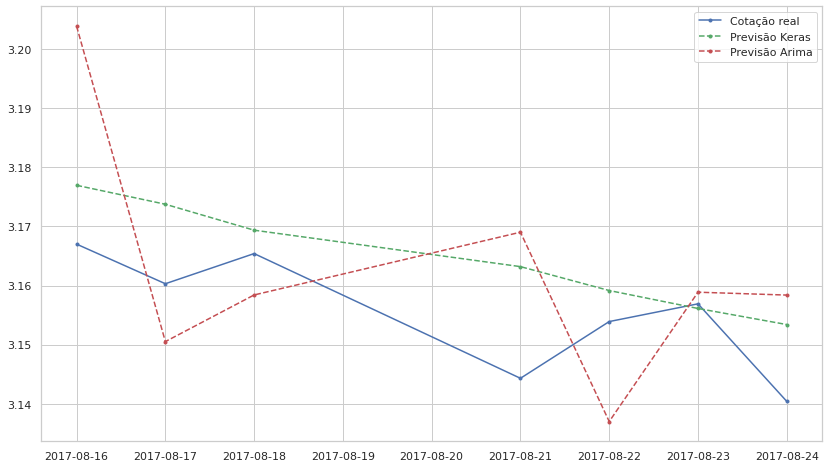
\includegraphics[width=14cm]{figuras/series_previsoes}
\caption{Previsões dos modelos ARIMA e Rede Neural (Keras) das janelas de cotações do Dólar.}
\label{fig:serie_previsoes}
\end{figure}